\documentclass[1p]{elsarticle_modified}
%\bibliographystyle{elsarticle-num}

%\usepackage[colorlinks]{hyperref}
%\usepackage{abbrmath_seonhwa} %\Abb, \Ascr, \Acal ,\Abf, \Afrak
\usepackage{amsfonts}
\usepackage{amssymb}
\usepackage{amsmath}
\usepackage{amsthm}
\usepackage{scalefnt}
\usepackage{amsbsy}
\usepackage{kotex}
\usepackage{caption}
\usepackage{subfig}
\usepackage{color}
\usepackage{graphicx}
\usepackage{xcolor} %% white, black, red, green, blue, cyan, magenta, yellow
\usepackage{float}
\usepackage{setspace}
\usepackage{hyperref}

\usepackage{tikz}
\usetikzlibrary{arrows}

\usepackage{multirow}
\usepackage{array} % fixed length table
\usepackage{hhline}

%%%%%%%%%%%%%%%%%%%%%
\makeatletter
\renewcommand*\env@matrix[1][\arraystretch]{%
	\edef\arraystretch{#1}%
	\hskip -\arraycolsep
	\let\@ifnextchar\new@ifnextchar
	\array{*\c@MaxMatrixCols c}}
\makeatother %https://tex.stackexchange.com/questions/14071/how-can-i-increase-the-line-spacing-in-a-matrix
%%%%%%%%%%%%%%%

\usepackage[normalem]{ulem}

\newcommand{\msout}[1]{\ifmmode\text{\sout{\ensuremath{#1}}}\else\sout{#1}\fi}
%SOURCE: \msout is \stkout macro in https://tex.stackexchange.com/questions/20609/strikeout-in-math-mode

\newcommand{\cancel}[1]{
	\ifmmode
	{\color{red}\msout{#1}}
	\else
	{\color{red}\sout{#1}}
	\fi
}

\newcommand{\add}[1]{
	{\color{blue}\uwave{#1}}
}

\newcommand{\replace}[2]{
	\ifmmode
	{\color{red}\msout{#1}}{\color{blue}\uwave{#2}}
	\else
	{\color{red}\sout{#1}}{\color{blue}\uwave{#2}}
	\fi
}

\newcommand{\Sol}{\mathcal{S}} %segment
\newcommand{\D}{D} %diagram
\newcommand{\A}{\mathcal{A}} %arc


%%%%%%%%%%%%%%%%%%%%%%%%%%%%%5 test

\def\sl{\operatorname{\textup{SL}}(2,\Cbb)}
\def\psl{\operatorname{\textup{PSL}}(2,\Cbb)}
\def\quan{\mkern 1mu \triangleright \mkern 1mu}

\theoremstyle{definition}
\newtheorem{thm}{Theorem}[section]
\newtheorem{prop}[thm]{Proposition}
\newtheorem{lem}[thm]{Lemma}
\newtheorem{ques}[thm]{Question}
\newtheorem{cor}[thm]{Corollary}
\newtheorem{defn}[thm]{Definition}
\newtheorem{exam}[thm]{Example}
\newtheorem{rmk}[thm]{Remark}
\newtheorem{alg}[thm]{Algorithm}

\newcommand{\I}{\sqrt{-1}}
\begin{document}

%\begin{frontmatter}
%
%\title{Boundary parabolic representations of knots up to 8 crossings}
%
%%% Group authors per affiliation:
%\author{Yunhi Cho} 
%\address{Department of Mathematics, University of Seoul, Seoul, Korea}
%\ead{yhcho@uos.ac.kr}
%
%
%\author{Seonhwa Kim} %\fnref{s_kim}}
%\address{Center for Geometry and Physics, Institute for Basic Science, Pohang, 37673, Korea}
%\ead{ryeona17@ibs.re.kr}
%
%\author{Hyuk Kim}
%\address{Department of Mathematical Sciences, Seoul National University, Seoul 08826, Korea}
%\ead{hyukkim@snu.ac.kr}
%
%\author{Seokbeom Yoon}
%\address{Department of Mathematical Sciences, Seoul National University, Seoul, 08826,  Korea}
%\ead{sbyoon15@snu.ac.kr}
%
%\begin{abstract}
%We find all boundary parabolic representation of knots up to 8 crossings.
%
%\end{abstract}
%\begin{keyword}
%    \MSC[2010] 57M25 
%\end{keyword}
%
%\end{frontmatter}

%\linenumbers
%\tableofcontents
%
\newcommand\colored[1]{\textcolor{white}{\rule[-0.35ex]{0.8em}{1.4ex}}\kern-0.8em\color{red} #1}%
%\newcommand\colored[1]{\textcolor{white}{ #1}\kern-2.17ex	\textcolor{white}{ #1}\kern-1.81ex	\textcolor{white}{ #1}\kern-2.15ex\color{red}#1	}

{\Large $\underline{12a_{1058}~(K12a_{1058})}$}

\setlength{\tabcolsep}{10pt}
\renewcommand{\arraystretch}{1.6}
\vspace{1cm}\begin{tabular}{m{100pt}>{\centering\arraybackslash}m{274pt}}
\multirow{5}{120pt}{
	\centering
	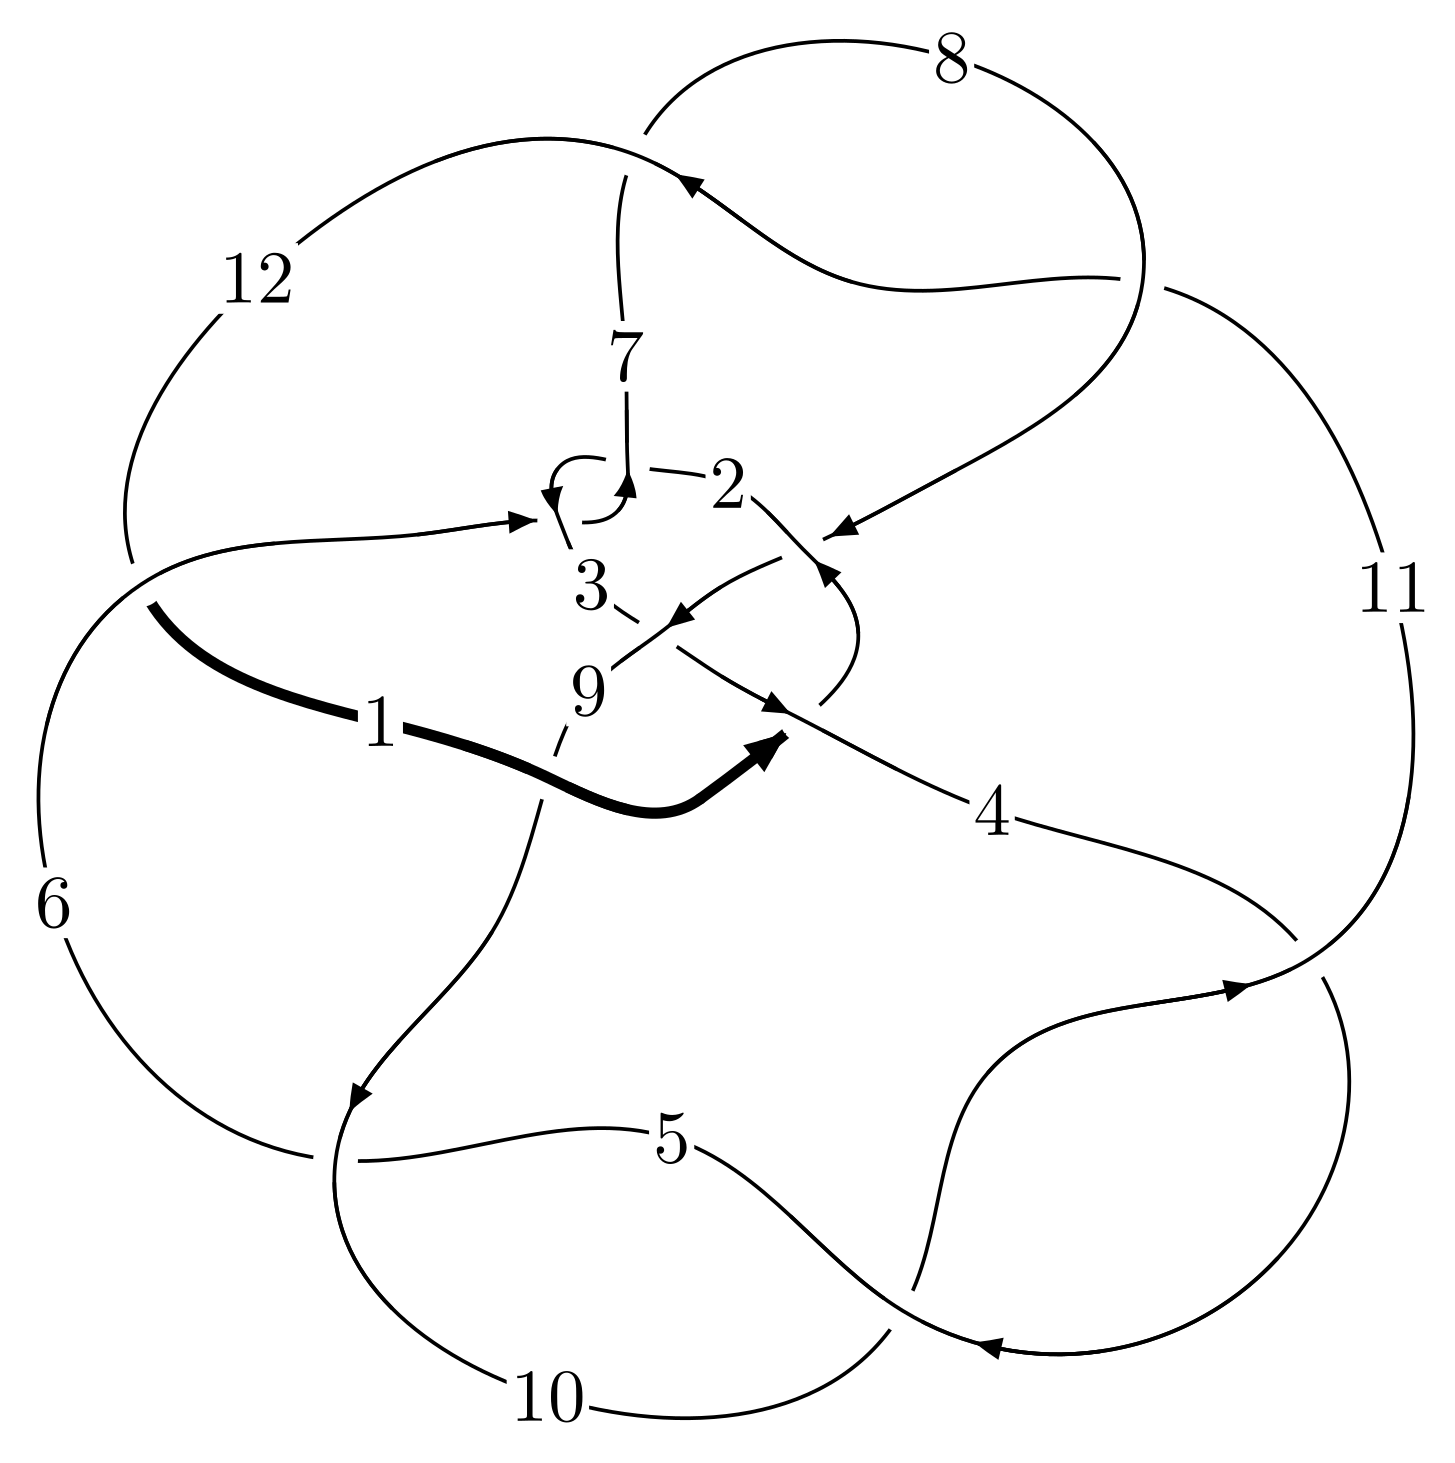
\includegraphics[width=112pt]{../../../GIT/diagram.site/Diagrams/png/1859_12a_1058.png}\\
\ \ \ A knot diagram\footnotemark}&
\allowdisplaybreaks
\textbf{Linearized knot diagam} \\
\cline{2-2}
 &
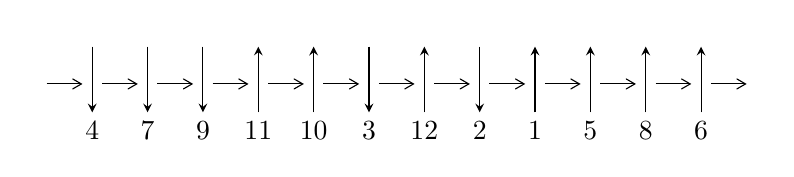
\begin{tikzpicture}[x=20pt, y=17pt]
	% nodes
	\node (C0) at (0, 0) {};
	\node (C1) at (1, 0) {};
	\node (C1U) at (1, +1) {};
	\node (C1D) at (1, -1) {4};

	\node (C2) at (2, 0) {};
	\node (C2U) at (2, +1) {};
	\node (C2D) at (2, -1) {7};

	\node (C3) at (3, 0) {};
	\node (C3U) at (3, +1) {};
	\node (C3D) at (3, -1) {9};

	\node (C4) at (4, 0) {};
	\node (C4U) at (4, +1) {};
	\node (C4D) at (4, -1) {11};

	\node (C5) at (5, 0) {};
	\node (C5U) at (5, +1) {};
	\node (C5D) at (5, -1) {10};

	\node (C6) at (6, 0) {};
	\node (C6U) at (6, +1) {};
	\node (C6D) at (6, -1) {3};

	\node (C7) at (7, 0) {};
	\node (C7U) at (7, +1) {};
	\node (C7D) at (7, -1) {12};

	\node (C8) at (8, 0) {};
	\node (C8U) at (8, +1) {};
	\node (C8D) at (8, -1) {2};

	\node (C9) at (9, 0) {};
	\node (C9U) at (9, +1) {};
	\node (C9D) at (9, -1) {1};

	\node (C10) at (10, 0) {};
	\node (C10U) at (10, +1) {};
	\node (C10D) at (10, -1) {5};

	\node (C11) at (11, 0) {};
	\node (C11U) at (11, +1) {};
	\node (C11D) at (11, -1) {8};

	\node (C12) at (12, 0) {};
	\node (C12U) at (12, +1) {};
	\node (C12D) at (12, -1) {6};
	\node (C13) at (13, 0) {};

	% arrows
	\draw[->,>={angle 60}]
	(C0) edge (C1) (C1) edge (C2) (C2) edge (C3) (C3) edge (C4) (C4) edge (C5) (C5) edge (C6) (C6) edge (C7) (C7) edge (C8) (C8) edge (C9) (C9) edge (C10) (C10) edge (C11) (C11) edge (C12) (C12) edge (C13) ;	\draw[->,>=stealth]
	(C1U) edge (C1D) (C2U) edge (C2D) (C3U) edge (C3D) (C4D) edge (C4U) (C5D) edge (C5U) (C6U) edge (C6D) (C7D) edge (C7U) (C8U) edge (C8D) (C9D) edge (C9U) (C10D) edge (C10U) (C11D) edge (C11U) (C12D) edge (C12U) ;
	\end{tikzpicture} \\
\hhline{~~} \\& 
\textbf{Solving Sequence} \\ \cline{2-2} 
 &
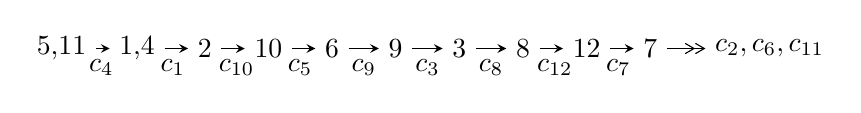
\begin{tikzpicture}[x=23pt, y=7pt]
	% node
	\node (A0) at (-1/8, 0) {5,11};
	\node (A1) at (17/16, 0) {1,4};
	\node (A2) at (17/8, 0) {2};
	\node (A3) at (25/8, 0) {10};
	\node (A4) at (33/8, 0) {6};
	\node (A5) at (41/8, 0) {9};
	\node (A6) at (49/8, 0) {3};
	\node (A7) at (57/8, 0) {8};
	\node (A8) at (65/8, 0) {12};
	\node (A9) at (73/8, 0) {7};
	\node (C1) at (1/2, -1) {$c_{4}$};
	\node (C2) at (13/8, -1) {$c_{1}$};
	\node (C3) at (21/8, -1) {$c_{10}$};
	\node (C4) at (29/8, -1) {$c_{5}$};
	\node (C5) at (37/8, -1) {$c_{9}$};
	\node (C6) at (45/8, -1) {$c_{3}$};
	\node (C7) at (53/8, -1) {$c_{8}$};
	\node (C8) at (61/8, -1) {$c_{12}$};
	\node (C9) at (69/8, -1) {$c_{7}$};
	\node (A10) at (11, 0) {$c_{2},c_{6},c_{11}$};

	% edge
	\draw[->,>=stealth]	
	(A0) edge (A1) (A1) edge (A2) (A2) edge (A3) (A3) edge (A4) (A4) edge (A5) (A5) edge (A6) (A6) edge (A7) (A7) edge (A8) (A8) edge (A9) ;
	\draw[->>,>={angle 60}]	
	(A9) edge (A10);
\end{tikzpicture} \\ 

\end{tabular} \\

\footnotetext{
The image of knot diagram is generated by the software ``\textbf{Draw programme}" developed by Andrew Bartholomew(\url{http://www.layer8.co.uk/maths/draw/index.htm\#Running-draw}), where we modified some parts for our purpose(\url{https://github.com/CATsTAILs/LinksPainter}).
}\phantom \\ \newline 
\centering \textbf{Ideals for irreducible components\footnotemark of $X_{\text{par}}$} 
 
\begin{align*}
I^u_{1}&=\langle 
6.77987\times10^{529} u^{151}-2.60638\times10^{530} u^{150}+\cdots+2.32236\times10^{530} b-7.75568\times10^{530},\\
\phantom{I^u_{1}}&\phantom{= \langle  }4.01232\times10^{530} u^{151}-1.86825\times10^{530} u^{150}+\cdots+6.96708\times10^{530} a-1.05433\times10^{532},\;u^{152}- u^{151}+\cdots-61 u+3\rangle \\
I^u_{2}&=\langle 
23135489547260 u^{41}-791878135073 u^{40}+\cdots+785779145393 b-1057448627428,\\
\phantom{I^u_{2}}&\phantom{= \langle  }-61366371188204 u^{41}-63826689923786 u^{40}+\cdots+3928895726965 a-80218304578144,\\
\phantom{I^u_{2}}&\phantom{= \langle  }u^{42}+23 u^{40}+\cdots+26 u^2+1\rangle \\
\\
\end{align*}
\raggedright * 2 irreducible components of $\dim_{\mathbb{C}}=0$, with total 194 representations.\\
\footnotetext{All coefficients of polynomials are rational numbers. But the coefficients are sometimes approximated in decimal forms when there is not enough margin.}
\newpage
\renewcommand{\arraystretch}{1}
\centering \section*{I. $I^u_{1}= \langle 6.78\times10^{529} u^{151}-2.61\times10^{530} u^{150}+\cdots+2.32\times10^{530} b-7.76\times10^{530},\;4.01\times10^{530} u^{151}-1.87\times10^{530} u^{150}+\cdots+6.97\times10^{530} a-1.05\times10^{532},\;u^{152}- u^{151}+\cdots-61 u+3 \rangle$}
\flushleft \textbf{(i) Arc colorings}\\
\begin{tabular}{m{7pt} m{180pt} m{7pt} m{180pt} }
\flushright $a_{5}=$&$\begin{pmatrix}1\\0\end{pmatrix}$ \\
\flushright $a_{11}=$&$\begin{pmatrix}0\\u\end{pmatrix}$ \\
\flushright $a_{1}=$&$\begin{pmatrix}-0.575897 u^{151}+0.268154 u^{150}+\cdots-218.578 u+15.1330\\-0.291939 u^{151}+1.12230 u^{150}+\cdots-58.3679 u+3.33957\end{pmatrix}$ \\
\flushright $a_{4}=$&$\begin{pmatrix}1\\u^2\end{pmatrix}$ \\
\flushright $a_{2}=$&$\begin{pmatrix}-0.188865 u^{151}-0.260558 u^{150}+\cdots-177.254 u+12.7167\\-0.542871 u^{151}+1.76489 u^{150}+\cdots-68.1715 u+3.76461\end{pmatrix}$ \\
\flushright $a_{10}=$&$\begin{pmatrix}- u\\u\end{pmatrix}$ \\
\flushright $a_{6}=$&$\begin{pmatrix}u^2+1\\- u^2\end{pmatrix}$ \\
\flushright $a_{9}=$&$\begin{pmatrix}-1.96213 u^{151}+0.333521 u^{150}+\cdots-400.771 u+20.0410\\-0.0536691 u^{151}+2.47127 u^{150}+\cdots+3.73527 u-1.95372\end{pmatrix}$ \\
\flushright $a_{3}=$&$\begin{pmatrix}7.33103 u^{151}-6.16852 u^{150}+\cdots+1895.49 u-129.107\\-0.954188 u^{151}+0.712754 u^{150}+\cdots+40.7323 u-2.82961\end{pmatrix}$ \\
\flushright $a_{8}=$&$\begin{pmatrix}0.535983 u^{151}-0.784566 u^{150}+\cdots+77.8051 u-8.33785\\0.0700948 u^{151}+0.756951 u^{150}+\cdots-52.3469 u+2.24342\end{pmatrix}$ \\
\flushright $a_{12}=$&$\begin{pmatrix}-0.203870 u^{151}-0.152271 u^{150}+\cdots-182.925 u+12.7787\\-0.638054 u^{151}+1.71099 u^{150}+\cdots-70.1352 u+3.92211\end{pmatrix}$ \\
\flushright $a_{7}=$&$\begin{pmatrix}-0.487296 u^{151}-0.705863 u^{150}+\cdots-34.0215 u-6.18471\\-0.0704317 u^{151}+2.34336 u^{150}+\cdots-31.4761 u+0.0244434\end{pmatrix}$\\&\end{tabular}
\flushleft \textbf{(ii) Obstruction class $= -1$}\\~\\
\flushleft \textbf{(iii) Cusp Shapes $= -0.0312083 u^{151}-1.55714 u^{150}+\cdots-167.321 u+31.3804$}\\~\\
\newpage\renewcommand{\arraystretch}{1}
\flushleft \textbf{(iv) u-Polynomials at the component}\newline \\
\begin{tabular}{m{50pt}|m{274pt}}
Crossings & \hspace{64pt}u-Polynomials at each crossing \\
\hline $$\begin{aligned}c_{1}\end{aligned}$$&$\begin{aligned}
&u^{152}-11 u^{151}+\cdots+18140 u+5351
\end{aligned}$\\
\hline $$\begin{aligned}c_{2},c_{6}\end{aligned}$$&$\begin{aligned}
&u^{152}- u^{151}+\cdots+4353 u+1651
\end{aligned}$\\
\hline $$\begin{aligned}c_{3}\end{aligned}$$&$\begin{aligned}
&u^{152}-2 u^{151}+\cdots+87 u+7
\end{aligned}$\\
\hline $$\begin{aligned}c_{4},c_{5},c_{10}\end{aligned}$$&$\begin{aligned}
&u^{152}+u^{151}+\cdots+61 u+3
\end{aligned}$\\
\hline $$\begin{aligned}c_{7},c_{11}\end{aligned}$$&$\begin{aligned}
&u^{152}+3 u^{151}+\cdots+61152 u+8128
\end{aligned}$\\
\hline $$\begin{aligned}c_{8}\end{aligned}$$&$\begin{aligned}
&u^{152}- u^{151}+\cdots+57030 u+6997
\end{aligned}$\\
\hline $$\begin{aligned}c_{9}\end{aligned}$$&$\begin{aligned}
&u^{152}-5 u^{151}+\cdots+176391091 u+46936013
\end{aligned}$\\
\hline $$\begin{aligned}c_{12}\end{aligned}$$&$\begin{aligned}
&u^{152}+u^{151}+\cdots-347000939 u+62972897
\end{aligned}$\\
\hline
\end{tabular}\\~\\
\newpage\renewcommand{\arraystretch}{1}
\flushleft \textbf{(v) Riley Polynomials at the component}\newline \\
\begin{tabular}{m{50pt}|m{274pt}}
Crossings & \hspace{64pt}Riley Polynomials at each crossing \\
\hline $$\begin{aligned}c_{1}\end{aligned}$$&$\begin{aligned}
&y^{152}-33 y^{151}+\cdots-1604598874 y+28633201
\end{aligned}$\\
\hline $$\begin{aligned}c_{2},c_{6}\end{aligned}$$&$\begin{aligned}
&y^{152}+83 y^{151}+\cdots+110545925 y+2725801
\end{aligned}$\\
\hline $$\begin{aligned}c_{3}\end{aligned}$$&$\begin{aligned}
&y^{152}-10 y^{151}+\cdots+3323 y+49
\end{aligned}$\\
\hline $$\begin{aligned}c_{4},c_{5},c_{10}\end{aligned}$$&$\begin{aligned}
&y^{152}+155 y^{151}+\cdots+275 y+9
\end{aligned}$\\
\hline $$\begin{aligned}c_{7},c_{11}\end{aligned}$$&$\begin{aligned}
&y^{152}+87 y^{151}+\cdots+2765433856 y+66064384
\end{aligned}$\\
\hline $$\begin{aligned}c_{8}\end{aligned}$$&$\begin{aligned}
&y^{152}+3 y^{151}+\cdots+3614155020 y+48958009
\end{aligned}$\\
\hline $$\begin{aligned}c_{9}\end{aligned}$$&$\begin{aligned}
&y^{152}+31 y^{151}+\cdots+104404411598711997 y+2202989316336169
\end{aligned}$\\
\hline $$\begin{aligned}c_{12}\end{aligned}$$&$\begin{aligned}
&y^{152}+47 y^{151}+\cdots+710392624054179195 y+3965585756572609
\end{aligned}$\\
\hline
\end{tabular}\\~\\
\newpage\flushleft \textbf{(vi) Complex Volumes and Cusp Shapes}
$$\begin{array}{c|c|c}  
\text{Solutions to }I^u_{1}& \I (\text{vol} + \sqrt{-1}CS) & \text{Cusp shape}\\
 \hline 
\begin{aligned}
u &= \phantom{-}0.878179 + 0.495642 I \\
a &= -0.564021 - 0.738126 I \\
b &= -0.752235 + 0.139735 I\end{aligned}
 & -0.7060 + 15.2759 I & \phantom{-0.000000 } 0 \\ \hline\begin{aligned}
u &= \phantom{-}0.878179 - 0.495642 I \\
a &= -0.564021 + 0.738126 I \\
b &= -0.752235 - 0.139735 I\end{aligned}
 & -0.7060 - 15.2759 I & \phantom{-0.000000 } 0 \\ \hline\begin{aligned}
u &= -0.886322 + 0.532057 I \\
a &= \phantom{-}0.420058 - 0.788913 I \\
b &= \phantom{-}0.644080 + 0.199211 I\end{aligned}
 & -3.72811 - 8.56360 I & \phantom{-0.000000 } 0 \\ \hline\begin{aligned}
u &= -0.886322 - 0.532057 I \\
a &= \phantom{-}0.420058 + 0.788913 I \\
b &= \phantom{-}0.644080 - 0.199211 I\end{aligned}
 & -3.72811 + 8.56360 I & \phantom{-0.000000 } 0 \\ \hline\begin{aligned}
u &= \phantom{-}0.116120 + 0.945775 I \\
a &= \phantom{-}0.457765 + 0.653681 I \\
b &= \phantom{-}0.169583 + 0.417592 I\end{aligned}
 & -2.65978 - 0.93404 I & \phantom{-0.000000 } 0 \\ \hline\begin{aligned}
u &= \phantom{-}0.116120 - 0.945775 I \\
a &= \phantom{-}0.457765 - 0.653681 I \\
b &= \phantom{-}0.169583 - 0.417592 I\end{aligned}
 & -2.65978 + 0.93404 I & \phantom{-0.000000 } 0 \\ \hline\begin{aligned}
u &= \phantom{-}0.407000 + 1.005930 I \\
a &= -0.437541 + 0.247181 I \\
b &= \phantom{-}0.810914 + 0.503999 I\end{aligned}
 & -1.70138 - 1.08051 I & \phantom{-0.000000 } 0 \\ \hline\begin{aligned}
u &= \phantom{-}0.407000 - 1.005930 I \\
a &= -0.437541 - 0.247181 I \\
b &= \phantom{-}0.810914 - 0.503999 I\end{aligned}
 & -1.70138 + 1.08051 I & \phantom{-0.000000 } 0 \\ \hline\begin{aligned}
u &= -0.742540 + 0.507978 I \\
a &= -0.884196 + 0.627862 I \\
b &= -0.601044 - 0.139088 I\end{aligned}
 & \phantom{-}2.69781 - 8.89406 I & \phantom{-0.000000 } 0 \\ \hline\begin{aligned}
u &= -0.742540 - 0.507978 I \\
a &= -0.884196 - 0.627862 I \\
b &= -0.601044 + 0.139088 I\end{aligned}
 & \phantom{-}2.69781 + 8.89406 I & \phantom{-0.000000 } 0\\
 \hline 
 \end{array}$$\newpage$$\begin{array}{c|c|c}  
\text{Solutions to }I^u_{1}& \I (\text{vol} + \sqrt{-1}CS) & \text{Cusp shape}\\
 \hline 
\begin{aligned}
u &= \phantom{-}0.833938 + 0.729054 I \\
a &= \phantom{-}0.193277 - 0.443729 I \\
b &= -0.445113 - 0.516791 I\end{aligned}
 & -1.33475 - 9.55748 I & \phantom{-0.000000 } 0 \\ \hline\begin{aligned}
u &= \phantom{-}0.833938 - 0.729054 I \\
a &= \phantom{-}0.193277 + 0.443729 I \\
b &= -0.445113 + 0.516791 I\end{aligned}
 & -1.33475 + 9.55748 I & \phantom{-0.000000 } 0 \\ \hline\begin{aligned}
u &= \phantom{-}0.788215 + 0.402245 I \\
a &= -0.397730 - 0.625511 I \\
b &= -0.252690 - 0.409109 I\end{aligned}
 & -3.76675 + 2.08728 I & \phantom{-0.000000 } 0 \\ \hline\begin{aligned}
u &= \phantom{-}0.788215 - 0.402245 I \\
a &= -0.397730 + 0.625511 I \\
b &= -0.252690 + 0.409109 I\end{aligned}
 & -3.76675 - 2.08728 I & \phantom{-0.000000 } 0 \\ \hline\begin{aligned}
u &= -0.430313 + 1.040840 I \\
a &= \phantom{-}0.505748 + 0.188593 I \\
b &= \phantom{-}0.216466 - 0.014818 I\end{aligned}
 & -2.69394 - 0.61392 I & \phantom{-0.000000 } 0 \\ \hline\begin{aligned}
u &= -0.430313 - 1.040840 I \\
a &= \phantom{-}0.505748 - 0.188593 I \\
b &= \phantom{-}0.216466 + 0.014818 I\end{aligned}
 & -2.69394 + 0.61392 I & \phantom{-0.000000 } 0 \\ \hline\begin{aligned}
u &= -0.718800 + 0.496615 I \\
a &= \phantom{-}0.239945 + 0.250970 I \\
b &= -0.306341 + 0.691719 I\end{aligned}
 & \phantom{-}2.65155 + 4.05569 I & \phantom{-0.000000 } 0 \\ \hline\begin{aligned}
u &= -0.718800 - 0.496615 I \\
a &= \phantom{-}0.239945 - 0.250970 I \\
b &= -0.306341 - 0.691719 I\end{aligned}
 & \phantom{-}2.65155 - 4.05569 I & \phantom{-0.000000 } 0 \\ \hline\begin{aligned}
u &= \phantom{-}0.765332 + 0.836222 I \\
a &= -0.496086 + 0.021099 I \\
b &= -0.410884 - 0.209396 I\end{aligned}
 & -3.70871 + 3.30219 I & \phantom{-0.000000 } 0 \\ \hline\begin{aligned}
u &= \phantom{-}0.765332 - 0.836222 I \\
a &= -0.496086 - 0.021099 I \\
b &= -0.410884 + 0.209396 I\end{aligned}
 & -3.70871 - 3.30219 I & \phantom{-0.000000 } 0\\
 \hline 
 \end{array}$$\newpage$$\begin{array}{c|c|c}  
\text{Solutions to }I^u_{1}& \I (\text{vol} + \sqrt{-1}CS) & \text{Cusp shape}\\
 \hline 
\begin{aligned}
u &= -0.866630 + 0.737689 I \\
a &= -0.257202 - 0.440095 I \\
b &= \phantom{-}0.595072 - 0.290409 I\end{aligned}
 & -4.23349 + 2.67967 I & \phantom{-0.000000 } 0 \\ \hline\begin{aligned}
u &= -0.866630 - 0.737689 I \\
a &= -0.257202 + 0.440095 I \\
b &= \phantom{-}0.595072 + 0.290409 I\end{aligned}
 & -4.23349 - 2.67967 I & \phantom{-0.000000 } 0 \\ \hline\begin{aligned}
u &= -0.798518 + 0.321414 I \\
a &= -0.403875 + 0.708676 I \\
b &= -0.678022 - 0.341985 I\end{aligned}
 & \phantom{-}3.00753 - 0.46886 I & \phantom{-0.000000 } 0 \\ \hline\begin{aligned}
u &= -0.798518 - 0.321414 I \\
a &= -0.403875 - 0.708676 I \\
b &= -0.678022 + 0.341985 I\end{aligned}
 & \phantom{-}3.00753 + 0.46886 I & \phantom{-0.000000 } 0 \\ \hline\begin{aligned}
u &= \phantom{-}0.010639 + 1.150670 I \\
a &= -0.122608 - 0.168471 I \\
b &= \phantom{-}0.389426 + 1.074840 I\end{aligned}
 & -1.53894 - 1.47676 I & \phantom{-0.000000 } 0 \\ \hline\begin{aligned}
u &= \phantom{-}0.010639 - 1.150670 I \\
a &= -0.122608 + 0.168471 I \\
b &= \phantom{-}0.389426 - 1.074840 I\end{aligned}
 & -1.53894 + 1.47676 I & \phantom{-0.000000 } 0 \\ \hline\begin{aligned}
u &= -0.670173 + 0.936099 I \\
a &= \phantom{-}0.182741 + 0.438576 I \\
b &= -0.168191 + 0.197395 I\end{aligned}
 & \phantom{-}1.30622 - 4.56377 I & \phantom{-0.000000 } 0 \\ \hline\begin{aligned}
u &= -0.670173 - 0.936099 I \\
a &= \phantom{-}0.182741 - 0.438576 I \\
b &= -0.168191 - 0.197395 I\end{aligned}
 & \phantom{-}1.30622 + 4.56377 I & \phantom{-0.000000 } 0 \\ \hline\begin{aligned}
u &= \phantom{-}0.885952 + 0.738183 I \\
a &= -0.031977 - 0.485715 I \\
b &= -0.452412 + 0.243336 I\end{aligned}
 & \phantom{-}4.23346 + 3.17237 I & \phantom{-0.000000 } 0 \\ \hline\begin{aligned}
u &= \phantom{-}0.885952 - 0.738183 I \\
a &= -0.031977 + 0.485715 I \\
b &= -0.452412 - 0.243336 I\end{aligned}
 & \phantom{-}4.23346 - 3.17237 I & \phantom{-0.000000 } 0\\
 \hline 
 \end{array}$$\newpage$$\begin{array}{c|c|c}  
\text{Solutions to }I^u_{1}& \I (\text{vol} + \sqrt{-1}CS) & \text{Cusp shape}\\
 \hline 
\begin{aligned}
u &= \phantom{-}0.632233 + 0.513263 I \\
a &= -0.939088 - 0.272049 I \\
b &= -0.621434 - 0.417344 I\end{aligned}
 & -4.29681 + 2.42359 I & \phantom{-0.000000 } 0 \\ \hline\begin{aligned}
u &= \phantom{-}0.632233 - 0.513263 I \\
a &= -0.939088 + 0.272049 I \\
b &= -0.621434 + 0.417344 I\end{aligned}
 & -4.29681 - 2.42359 I & \phantom{-0.000000 } 0 \\ \hline\begin{aligned}
u &= -0.205898 + 1.186000 I \\
a &= -0.582756 + 0.982859 I \\
b &= \phantom{-}0.447247 + 0.094284 I\end{aligned}
 & -1.65459 + 3.47179 I & \phantom{-0.000000 } 0 \\ \hline\begin{aligned}
u &= -0.205898 - 1.186000 I \\
a &= -0.582756 - 0.982859 I \\
b &= \phantom{-}0.447247 - 0.094284 I\end{aligned}
 & -1.65459 - 3.47179 I & \phantom{-0.000000 } 0 \\ \hline\begin{aligned}
u &= -1.139650 + 0.433163 I \\
a &= \phantom{-}0.116838 - 0.194203 I \\
b &= \phantom{-}0.262431 - 0.162027 I\end{aligned}
 & \phantom{-}0.03737 - 5.44081 I & \phantom{-0.000000 } 0 \\ \hline\begin{aligned}
u &= -1.139650 - 0.433163 I \\
a &= \phantom{-}0.116838 + 0.194203 I \\
b &= \phantom{-}0.262431 + 0.162027 I\end{aligned}
 & \phantom{-}0.03737 + 5.44081 I & \phantom{-0.000000 } 0 \\ \hline\begin{aligned}
u &= \phantom{-}0.410672 + 0.652255 I \\
a &= -0.293315 - 0.129450 I \\
b &= -0.508365 + 0.769709 I\end{aligned}
 & \phantom{-}4.54413 + 3.63997 I & \phantom{-0.000000 } 0 \\ \hline\begin{aligned}
u &= \phantom{-}0.410672 - 0.652255 I \\
a &= -0.293315 + 0.129450 I \\
b &= -0.508365 - 0.769709 I\end{aligned}
 & \phantom{-}4.54413 - 3.63997 I & \phantom{-0.000000 } 0 \\ \hline\begin{aligned}
u &= \phantom{-}0.652917 + 0.400077 I \\
a &= \phantom{-}0.875931 + 0.919214 I \\
b &= \phantom{-}0.587310 - 0.280434 I\end{aligned}
 & -0.37881 + 4.59426 I & \phantom{-0.000000 } 0 \\ \hline\begin{aligned}
u &= \phantom{-}0.652917 - 0.400077 I \\
a &= \phantom{-}0.875931 - 0.919214 I \\
b &= \phantom{-}0.587310 + 0.280434 I\end{aligned}
 & -0.37881 - 4.59426 I & \phantom{-0.000000 } 0\\
 \hline 
 \end{array}$$\newpage$$\begin{array}{c|c|c}  
\text{Solutions to }I^u_{1}& \I (\text{vol} + \sqrt{-1}CS) & \text{Cusp shape}\\
 \hline 
\begin{aligned}
u &= \phantom{-}0.129057 + 0.740489 I \\
a &= -0.559667 + 0.791209 I \\
b &= \phantom{-}1.23420 - 0.86120 I\end{aligned}
 & -3.38245 - 1.15411 I & \phantom{-0.000000 } 0 \\ \hline\begin{aligned}
u &= \phantom{-}0.129057 - 0.740489 I \\
a &= -0.559667 - 0.791209 I \\
b &= \phantom{-}1.23420 + 0.86120 I\end{aligned}
 & -3.38245 + 1.15411 I & \phantom{-0.000000 } 0 \\ \hline\begin{aligned}
u &= \phantom{-}0.154921 + 1.244210 I \\
a &= \phantom{-}1.49381 + 0.02502 I \\
b &= -1.42953 - 0.41635 I\end{aligned}
 & -3.34546 + 5.16441 I & \phantom{-0.000000 } 0 \\ \hline\begin{aligned}
u &= \phantom{-}0.154921 - 1.244210 I \\
a &= \phantom{-}1.49381 - 0.02502 I \\
b &= -1.42953 + 0.41635 I\end{aligned}
 & -3.34546 - 5.16441 I & \phantom{-0.000000 } 0 \\ \hline\begin{aligned}
u &= \phantom{-}0.731029 + 0.077477 I \\
a &= -0.292731 - 0.205590 I \\
b &= \phantom{-}0.480046 + 0.669669 I\end{aligned}
 & \phantom{-}0.06364 - 2.09801 I & \phantom{-0.000000 } 0 \\ \hline\begin{aligned}
u &= \phantom{-}0.731029 - 0.077477 I \\
a &= -0.292731 + 0.205590 I \\
b &= \phantom{-}0.480046 - 0.669669 I\end{aligned}
 & \phantom{-}0.06364 + 2.09801 I & \phantom{-0.000000 } 0 \\ \hline\begin{aligned}
u &= -0.698365 + 0.208979 I \\
a &= -0.248960 - 1.215250 I \\
b &= -0.079980 - 0.434451 I\end{aligned}
 & -1.64281 + 2.39766 I & \phantom{-0.000000 } 0 \\ \hline\begin{aligned}
u &= -0.698365 - 0.208979 I \\
a &= -0.248960 + 1.215250 I \\
b &= -0.079980 + 0.434451 I\end{aligned}
 & -1.64281 - 2.39766 I & \phantom{-0.000000 } 0 \\ \hline\begin{aligned}
u &= \phantom{-}0.070858 + 1.275140 I \\
a &= \phantom{-}2.26182 + 0.52413 I \\
b &= -3.71114 - 0.78285 I\end{aligned}
 & -1.83616 + 7.02854 I & \phantom{-0.000000 } 0 \\ \hline\begin{aligned}
u &= \phantom{-}0.070858 - 1.275140 I \\
a &= \phantom{-}2.26182 - 0.52413 I \\
b &= -3.71114 + 0.78285 I\end{aligned}
 & -1.83616 - 7.02854 I & \phantom{-0.000000 } 0\\
 \hline 
 \end{array}$$\newpage$$\begin{array}{c|c|c}  
\text{Solutions to }I^u_{1}& \I (\text{vol} + \sqrt{-1}CS) & \text{Cusp shape}\\
 \hline 
\begin{aligned}
u &= \phantom{-}0.410942 + 0.550754 I \\
a &= \phantom{-}0.774903 - 1.136430 I \\
b &= \phantom{-}0.112360 - 0.223213 I\end{aligned}
 & \phantom{-}4.73178 - 0.42762 I & \phantom{-0.000000 } 0 \\ \hline\begin{aligned}
u &= \phantom{-}0.410942 - 0.550754 I \\
a &= \phantom{-}0.774903 + 1.136430 I \\
b &= \phantom{-}0.112360 + 0.223213 I\end{aligned}
 & \phantom{-}4.73178 + 0.42762 I & \phantom{-0.000000 } 0 \\ \hline\begin{aligned}
u &= -0.115670 + 1.319870 I \\
a &= -1.36451 + 0.88061 I \\
b &= \phantom{-}2.23719 - 0.43979 I\end{aligned}
 & -4.80210 - 4.79919 I & \phantom{-0.000000 } 0 \\ \hline\begin{aligned}
u &= -0.115670 - 1.319870 I \\
a &= -1.36451 - 0.88061 I \\
b &= \phantom{-}2.23719 + 0.43979 I\end{aligned}
 & -4.80210 + 4.79919 I & \phantom{-0.000000 } 0 \\ \hline\begin{aligned}
u &= \phantom{-}0.208472 + 1.310300 I \\
a &= \phantom{-}0.89939 + 1.17267 I \\
b &= -1.58138 - 1.27280 I\end{aligned}
 & -6.08306 + 0.50528 I & \phantom{-0.000000 } 0 \\ \hline\begin{aligned}
u &= \phantom{-}0.208472 - 1.310300 I \\
a &= \phantom{-}0.89939 - 1.17267 I \\
b &= -1.58138 + 1.27280 I\end{aligned}
 & -6.08306 - 0.50528 I & \phantom{-0.000000 } 0 \\ \hline\begin{aligned}
u &= -0.508578 + 0.431740 I \\
a &= \phantom{-}1.248810 + 0.056768 I \\
b &= \phantom{-}1.009340 - 0.226090 I\end{aligned}
 & -2.52055 - 5.73891 I & \phantom{-0.000000 } 0 \\ \hline\begin{aligned}
u &= -0.508578 - 0.431740 I \\
a &= \phantom{-}1.248810 - 0.056768 I \\
b &= \phantom{-}1.009340 + 0.226090 I\end{aligned}
 & -2.52055 + 5.73891 I & \phantom{-0.000000 } 0 \\ \hline\begin{aligned}
u &= -0.133462 + 1.331980 I \\
a &= -2.90036 - 0.13099 I \\
b &= \phantom{-}3.26439 + 0.50437 I\end{aligned}
 & -2.23942 - 8.63079 I & \phantom{-0.000000 } 0 \\ \hline\begin{aligned}
u &= -0.133462 - 1.331980 I \\
a &= -2.90036 + 0.13099 I \\
b &= \phantom{-}3.26439 - 0.50437 I\end{aligned}
 & -2.23942 + 8.63079 I & \phantom{-0.000000 } 0\\
 \hline 
 \end{array}$$\newpage$$\begin{array}{c|c|c}  
\text{Solutions to }I^u_{1}& \I (\text{vol} + \sqrt{-1}CS) & \text{Cusp shape}\\
 \hline 
\begin{aligned}
u &= \phantom{-}0.033696 + 1.350720 I \\
a &= \phantom{-}1.70640 - 0.85038 I \\
b &= -2.82792 + 1.64885 I\end{aligned}
 & -0.265313 - 0.091703 I & \phantom{-0.000000 } 0 \\ \hline\begin{aligned}
u &= \phantom{-}0.033696 - 1.350720 I \\
a &= \phantom{-}1.70640 + 0.85038 I \\
b &= -2.82792 - 1.64885 I\end{aligned}
 & -0.265313 + 0.091703 I & \phantom{-0.000000 } 0 \\ \hline\begin{aligned}
u &= \phantom{-}0.606994 + 0.220097 I \\
a &= \phantom{-}0.89141 + 1.16253 I \\
b &= \phantom{-}0.933696 - 0.308841 I\end{aligned}
 & -0.49470 + 3.84426 I & \phantom{-0.000000 } 0 \\ \hline\begin{aligned}
u &= \phantom{-}0.606994 - 0.220097 I \\
a &= \phantom{-}0.89141 - 1.16253 I \\
b &= \phantom{-}0.933696 + 0.308841 I\end{aligned}
 & -0.49470 - 3.84426 I & \phantom{-0.000000 } 0 \\ \hline\begin{aligned}
u &= \phantom{-}0.642477 + 0.029689 I \\
a &= \phantom{-}0.48324 - 2.08567 I \\
b &= \phantom{-}0.310626 + 0.240849 I\end{aligned}
 & \phantom{-}1.51598 - 4.61783 I & \phantom{-}7.58913 + 6.56112 I \\ \hline\begin{aligned}
u &= \phantom{-}0.642477 - 0.029689 I \\
a &= \phantom{-}0.48324 + 2.08567 I \\
b &= \phantom{-}0.310626 - 0.240849 I\end{aligned}
 & \phantom{-}1.51598 + 4.61783 I & \phantom{-}7.58913 - 6.56112 I \\ \hline\begin{aligned}
u &= -0.115573 + 1.361180 I \\
a &= -1.58752 + 0.07873 I \\
b &= \phantom{-}2.50751 + 0.05649 I\end{aligned}
 & -3.72991 - 2.68509 I & \phantom{-0.000000 } 0 \\ \hline\begin{aligned}
u &= -0.115573 - 1.361180 I \\
a &= -1.58752 - 0.07873 I \\
b &= \phantom{-}2.50751 - 0.05649 I\end{aligned}
 & -3.72991 + 2.68509 I & \phantom{-0.000000 } 0 \\ \hline\begin{aligned}
u &= \phantom{-}0.001948 + 1.367560 I \\
a &= -0.634661 - 1.006570 I \\
b &= \phantom{-}0.565920 + 0.136836 I\end{aligned}
 & -0.09493 - 3.07336 I & \phantom{-0.000000 } 0 \\ \hline\begin{aligned}
u &= \phantom{-}0.001948 - 1.367560 I \\
a &= -0.634661 + 1.006570 I \\
b &= \phantom{-}0.565920 - 0.136836 I\end{aligned}
 & -0.09493 + 3.07336 I & \phantom{-0.000000 } 0\\
 \hline 
 \end{array}$$\newpage$$\begin{array}{c|c|c}  
\text{Solutions to }I^u_{1}& \I (\text{vol} + \sqrt{-1}CS) & \text{Cusp shape}\\
 \hline 
\begin{aligned}
u &= \phantom{-}0.314984 + 0.538551 I \\
a &= \phantom{-}0.411245 + 0.685565 I \\
b &= -1.51127 - 0.96772 I\end{aligned}
 & -0.56290 + 7.37137 I & -3.06670 - 12.47022 I \\ \hline\begin{aligned}
u &= \phantom{-}0.314984 - 0.538551 I \\
a &= \phantom{-}0.411245 - 0.685565 I \\
b &= -1.51127 + 0.96772 I\end{aligned}
 & -0.56290 - 7.37137 I & -3.06670 + 12.47022 I \\ \hline\begin{aligned}
u &= -0.184310 + 1.363750 I \\
a &= -1.44372 + 0.49130 I \\
b &= \phantom{-}2.33228 - 1.00507 I\end{aligned}
 & -3.12222 - 3.03364 I & \phantom{-0.000000 } 0 \\ \hline\begin{aligned}
u &= -0.184310 - 1.363750 I \\
a &= -1.44372 - 0.49130 I \\
b &= \phantom{-}2.33228 + 1.00507 I\end{aligned}
 & -3.12222 + 3.03364 I & \phantom{-0.000000 } 0 \\ \hline\begin{aligned}
u &= \phantom{-}0.037332 + 1.388960 I \\
a &= -0.202938 - 0.969776 I \\
b &= \phantom{-}0.46607 + 2.80907 I\end{aligned}
 & -0.46634 + 1.58117 I & \phantom{-0.000000 } 0 \\ \hline\begin{aligned}
u &= \phantom{-}0.037332 - 1.388960 I \\
a &= -0.202938 + 0.969776 I \\
b &= \phantom{-}0.46607 - 2.80907 I\end{aligned}
 & -0.46634 - 1.58117 I & \phantom{-0.000000 } 0 \\ \hline\begin{aligned}
u &= -0.538277 + 0.262771 I \\
a &= -0.50775 + 1.86121 I \\
b &= -0.204069 - 0.084432 I\end{aligned}
 & \phantom{-}1.97803 - 0.38146 I & \phantom{-}5.59987 + 4.41528 I \\ \hline\begin{aligned}
u &= -0.538277 - 0.262771 I \\
a &= -0.50775 - 1.86121 I \\
b &= -0.204069 + 0.084432 I\end{aligned}
 & \phantom{-}1.97803 + 0.38146 I & \phantom{-}5.59987 - 4.41528 I \\ \hline\begin{aligned}
u &= \phantom{-}0.060103 + 1.402450 I \\
a &= -2.24427 + 0.88372 I \\
b &= \phantom{-}2.67619 - 1.09906 I\end{aligned}
 & -1.05714 + 4.17647 I & \phantom{-0.000000 } 0 \\ \hline\begin{aligned}
u &= \phantom{-}0.060103 - 1.402450 I \\
a &= -2.24427 - 0.88372 I \\
b &= \phantom{-}2.67619 + 1.09906 I\end{aligned}
 & -1.05714 - 4.17647 I & \phantom{-0.000000 } 0\\
 \hline 
 \end{array}$$\newpage$$\begin{array}{c|c|c}  
\text{Solutions to }I^u_{1}& \I (\text{vol} + \sqrt{-1}CS) & \text{Cusp shape}\\
 \hline 
\begin{aligned}
u &= -0.424518 + 0.417116 I \\
a &= -0.126083 + 0.185627 I \\
b &= -0.994890 + 0.501376 I\end{aligned}
 & \phantom{-}1.37417 - 2.63932 I & \phantom{-}1.62166 + 6.27105 I \\ \hline\begin{aligned}
u &= -0.424518 - 0.417116 I \\
a &= -0.126083 - 0.185627 I \\
b &= -0.994890 - 0.501376 I\end{aligned}
 & \phantom{-}1.37417 + 2.63932 I & \phantom{-}1.62166 - 6.27105 I \\ \hline\begin{aligned}
u &= \phantom{-}0.230894 + 1.392570 I \\
a &= \phantom{-}2.28908 + 0.15368 I \\
b &= -3.24032 + 0.31085 I\end{aligned}
 & -5.66371 + 6.89455 I & \phantom{-0.000000 } 0 \\ \hline\begin{aligned}
u &= \phantom{-}0.230894 - 1.392570 I \\
a &= \phantom{-}2.28908 - 0.15368 I \\
b &= -3.24032 - 0.31085 I\end{aligned}
 & -5.66371 - 6.89455 I & \phantom{-0.000000 } 0 \\ \hline\begin{aligned}
u &= \phantom{-}0.02625 + 1.41853 I \\
a &= \phantom{-}1.66091 + 1.08394 I \\
b &= -2.30521 - 0.97878 I\end{aligned}
 & -6.80026 - 0.18763 I & \phantom{-0.000000 } 0 \\ \hline\begin{aligned}
u &= \phantom{-}0.02625 - 1.41853 I \\
a &= \phantom{-}1.66091 - 1.08394 I \\
b &= -2.30521 + 0.97878 I\end{aligned}
 & -6.80026 + 0.18763 I & \phantom{-0.000000 } 0 \\ \hline\begin{aligned}
u &= \phantom{-}0.08600 + 1.41972 I \\
a &= \phantom{-}0.283142 + 0.341148 I \\
b &= -0.38647 - 1.70858 I\end{aligned}
 & -6.76026 + 4.33959 I & \phantom{-0.000000 } 0 \\ \hline\begin{aligned}
u &= \phantom{-}0.08600 - 1.41972 I \\
a &= \phantom{-}0.283142 - 0.341148 I \\
b &= -0.38647 + 1.70858 I\end{aligned}
 & -6.76026 - 4.33959 I & \phantom{-0.000000 } 0 \\ \hline\begin{aligned}
u &= -0.14412 + 1.42704 I \\
a &= -1.50627 + 0.96619 I \\
b &= \phantom{-}2.16922 - 0.64576 I\end{aligned}
 & -4.51801 - 4.72556 I & \phantom{-0.000000 } 0 \\ \hline\begin{aligned}
u &= -0.14412 - 1.42704 I \\
a &= -1.50627 - 0.96619 I \\
b &= \phantom{-}2.16922 + 0.64576 I\end{aligned}
 & -4.51801 + 4.72556 I & \phantom{-0.000000 } 0\\
 \hline 
 \end{array}$$\newpage$$\begin{array}{c|c|c}  
\text{Solutions to }I^u_{1}& \I (\text{vol} + \sqrt{-1}CS) & \text{Cusp shape}\\
 \hline 
\begin{aligned}
u &= -0.11819 + 1.43236 I \\
a &= -0.445663 + 0.854091 I \\
b &= \phantom{-}0.91778 - 2.49354 I\end{aligned}
 & -4.84175 - 9.29715 I & \phantom{-0.000000 } 0 \\ \hline\begin{aligned}
u &= -0.11819 - 1.43236 I \\
a &= -0.445663 - 0.854091 I \\
b &= \phantom{-}0.91778 + 2.49354 I\end{aligned}
 & -4.84175 + 9.29715 I & \phantom{-0.000000 } 0 \\ \hline\begin{aligned}
u &= -0.552765 + 0.014313 I \\
a &= -0.551912 + 0.994139 I \\
b &= -1.33289 - 0.60978 I\end{aligned}
 & \phantom{-}1.92935 - 6.33185 I & \phantom{-}7.17773 + 7.64906 I \\ \hline\begin{aligned}
u &= -0.552765 - 0.014313 I \\
a &= -0.551912 - 0.994139 I \\
b &= -1.33289 + 0.60978 I\end{aligned}
 & \phantom{-}1.92935 + 6.33185 I & \phantom{-}7.17773 - 7.64906 I \\ \hline\begin{aligned}
u &= -0.02545 + 1.44803 I \\
a &= -0.857855 - 0.915020 I \\
b &= \phantom{-}1.379970 + 0.195468 I\end{aligned}
 & -7.80468 + 0.57106 I & \phantom{-0.000000 } 0 \\ \hline\begin{aligned}
u &= -0.02545 - 1.44803 I \\
a &= -0.857855 + 0.915020 I \\
b &= \phantom{-}1.379970 - 0.195468 I\end{aligned}
 & -7.80468 - 0.57106 I & \phantom{-0.000000 } 0 \\ \hline\begin{aligned}
u &= \phantom{-}0.265503 + 0.474764 I \\
a &= \phantom{-}0.044541 + 0.548942 I \\
b &= \phantom{-}0.493979 + 0.594564 I\end{aligned}
 & -1.19022 - 1.06033 I & -1.73863 + 1.28370 I \\ \hline\begin{aligned}
u &= \phantom{-}0.265503 - 0.474764 I \\
a &= \phantom{-}0.044541 - 0.548942 I \\
b &= \phantom{-}0.493979 - 0.594564 I\end{aligned}
 & -1.19022 + 1.06033 I & -1.73863 - 1.28370 I \\ \hline\begin{aligned}
u &= \phantom{-}0.08657 + 1.45661 I \\
a &= \phantom{-}1.79739 - 0.84767 I \\
b &= -2.52447 + 0.59620 I\end{aligned}
 & -7.94583 + 5.57874 I & \phantom{-0.000000 } 0 \\ \hline\begin{aligned}
u &= \phantom{-}0.08657 - 1.45661 I \\
a &= \phantom{-}1.79739 + 0.84767 I \\
b &= -2.52447 - 0.59620 I\end{aligned}
 & -7.94583 - 5.57874 I & \phantom{-0.000000 } 0\\
 \hline 
 \end{array}$$\newpage$$\begin{array}{c|c|c}  
\text{Solutions to }I^u_{1}& \I (\text{vol} + \sqrt{-1}CS) & \text{Cusp shape}\\
 \hline 
\begin{aligned}
u &= -0.28382 + 1.43940 I \\
a &= -1.78343 + 0.10037 I \\
b &= \phantom{-}2.50470 + 0.23320 I\end{aligned}
 & -2.63550 - 4.32707 I & \phantom{-0.000000 } 0 \\ \hline\begin{aligned}
u &= -0.28382 - 1.43940 I \\
a &= -1.78343 - 0.10037 I \\
b &= \phantom{-}2.50470 - 0.23320 I\end{aligned}
 & -2.63550 + 4.32707 I & \phantom{-0.000000 } 0 \\ \hline\begin{aligned}
u &= -0.32556 + 1.43576 I \\
a &= \phantom{-}0.786718 - 0.659743 I \\
b &= -1.61784 + 0.97399 I\end{aligned}
 & -6.90278 - 1.49526 I & \phantom{-0.000000 } 0 \\ \hline\begin{aligned}
u &= -0.32556 - 1.43576 I \\
a &= \phantom{-}0.786718 + 0.659743 I \\
b &= -1.61784 - 0.97399 I\end{aligned}
 & -6.90278 + 1.49526 I & \phantom{-0.000000 } 0 \\ \hline\begin{aligned}
u &= -0.19290 + 1.46908 I \\
a &= \phantom{-}1.95452 - 0.08392 I \\
b &= -3.03246 - 0.75220 I\end{aligned}
 & -8.68740 - 8.37475 I & \phantom{-0.000000 } 0 \\ \hline\begin{aligned}
u &= -0.19290 - 1.46908 I \\
a &= \phantom{-}1.95452 + 0.08392 I \\
b &= -3.03246 + 0.75220 I\end{aligned}
 & -8.68740 + 8.37475 I & \phantom{-0.000000 } 0 \\ \hline\begin{aligned}
u &= -0.492386 + 0.154953 I \\
a &= -1.074880 + 0.699992 I \\
b &= -0.280796 - 0.145558 I\end{aligned}
 & \phantom{-}1.040050 - 0.549467 I & \phantom{-}7.43364 + 2.00474 I \\ \hline\begin{aligned}
u &= -0.492386 - 0.154953 I \\
a &= -1.074880 - 0.699992 I \\
b &= -0.280796 + 0.145558 I\end{aligned}
 & \phantom{-}1.040050 + 0.549467 I & \phantom{-}7.43364 - 2.00474 I \\ \hline\begin{aligned}
u &= \phantom{-}0.23108 + 1.48576 I \\
a &= \phantom{-}1.88952 - 0.11064 I \\
b &= -2.90807 + 0.43693 I\end{aligned}
 & -6.55064 + 7.81946 I & \phantom{-0.000000 } 0 \\ \hline\begin{aligned}
u &= \phantom{-}0.23108 - 1.48576 I \\
a &= \phantom{-}1.88952 + 0.11064 I \\
b &= -2.90807 - 0.43693 I\end{aligned}
 & -6.55064 - 7.81946 I & \phantom{-0.000000 } 0\\
 \hline 
 \end{array}$$\newpage$$\begin{array}{c|c|c}  
\text{Solutions to }I^u_{1}& \I (\text{vol} + \sqrt{-1}CS) & \text{Cusp shape}\\
 \hline 
\begin{aligned}
u &= \phantom{-}0.22737 + 1.49355 I \\
a &= -1.69122 - 0.29947 I \\
b &= \phantom{-}3.00950 - 0.23740 I\end{aligned}
 & -10.78190 + 5.59014 I & \phantom{-0.000000 } 0 \\ \hline\begin{aligned}
u &= \phantom{-}0.22737 - 1.49355 I \\
a &= -1.69122 + 0.29947 I \\
b &= \phantom{-}3.00950 + 0.23740 I\end{aligned}
 & -10.78190 - 5.59014 I & \phantom{-0.000000 } 0 \\ \hline\begin{aligned}
u &= \phantom{-}0.12929 + 1.51346 I \\
a &= -1.47261 - 1.46945 I \\
b &= \phantom{-}1.90290 + 1.11091 I\end{aligned}
 & -7.32672 + 9.14085 I & \phantom{-0.000000 } 0 \\ \hline\begin{aligned}
u &= \phantom{-}0.12929 - 1.51346 I \\
a &= -1.47261 + 1.46945 I \\
b &= \phantom{-}1.90290 - 1.11091 I\end{aligned}
 & -7.32672 - 9.14085 I & \phantom{-0.000000 } 0 \\ \hline\begin{aligned}
u &= -0.26396 + 1.52000 I \\
a &= -1.78890 - 0.10389 I \\
b &= \phantom{-}2.87925 + 0.58891 I\end{aligned}
 & -3.90420 - 12.58760 I & \phantom{-0.000000 } 0 \\ \hline\begin{aligned}
u &= -0.26396 - 1.52000 I \\
a &= -1.78890 + 0.10389 I \\
b &= \phantom{-}2.87925 - 0.58891 I\end{aligned}
 & -3.90420 + 12.58760 I & \phantom{-0.000000 } 0 \\ \hline\begin{aligned}
u &= \phantom{-}0.30619 + 1.51476 I \\
a &= -1.104380 - 0.300115 I \\
b &= \phantom{-}2.02876 + 0.09939 I\end{aligned}
 & -10.02160 + 6.17791 I & \phantom{-0.000000 } 0 \\ \hline\begin{aligned}
u &= \phantom{-}0.30619 - 1.51476 I \\
a &= -1.104380 + 0.300115 I \\
b &= \phantom{-}2.02876 - 0.09939 I\end{aligned}
 & -10.02160 - 6.17791 I & \phantom{-0.000000 } 0 \\ \hline\begin{aligned}
u &= -0.11442 + 1.55249 I \\
a &= \phantom{-}1.63445 + 0.36014 I \\
b &= -2.66201 - 0.79590 I\end{aligned}
 & -10.77330 - 2.23854 I & \phantom{-0.000000 } 0 \\ \hline\begin{aligned}
u &= -0.11442 - 1.55249 I \\
a &= \phantom{-}1.63445 - 0.36014 I \\
b &= -2.66201 + 0.79590 I\end{aligned}
 & -10.77330 + 2.23854 I & \phantom{-0.000000 } 0\\
 \hline 
 \end{array}$$\newpage$$\begin{array}{c|c|c}  
\text{Solutions to }I^u_{1}& \I (\text{vol} + \sqrt{-1}CS) & \text{Cusp shape}\\
 \hline 
\begin{aligned}
u &= \phantom{-}0.31801 + 1.53267 I \\
a &= -1.80409 - 0.05058 I \\
b &= \phantom{-}2.84291 - 0.42225 I\end{aligned}
 & -7.2738 + 19.6356 I & \phantom{-0.000000 } 0 \\ \hline\begin{aligned}
u &= \phantom{-}0.31801 - 1.53267 I \\
a &= -1.80409 + 0.05058 I \\
b &= \phantom{-}2.84291 + 0.42225 I\end{aligned}
 & -7.2738 - 19.6356 I & \phantom{-0.000000 } 0 \\ \hline\begin{aligned}
u &= -0.340179 + 0.267909 I \\
a &= \phantom{-}0.92686 + 4.13715 I \\
b &= \phantom{-}0.350396 - 0.479965 I\end{aligned}
 & \phantom{-}0.73173 - 7.59496 I & \phantom{-}6.6801 + 14.7598 I \\ \hline\begin{aligned}
u &= -0.340179 - 0.267909 I \\
a &= \phantom{-}0.92686 - 4.13715 I \\
b &= \phantom{-}0.350396 + 0.479965 I\end{aligned}
 & \phantom{-}0.73173 + 7.59496 I & \phantom{-}6.6801 - 14.7598 I \\ \hline\begin{aligned}
u &= -0.31033 + 1.54831 I \\
a &= \phantom{-}1.74043 - 0.02740 I \\
b &= -2.71337 - 0.30230 I\end{aligned}
 & -10.4891 - 12.9239 I & \phantom{-0.000000 } 0 \\ \hline\begin{aligned}
u &= -0.31033 - 1.54831 I \\
a &= \phantom{-}1.74043 + 0.02740 I \\
b &= -2.71337 + 0.30230 I\end{aligned}
 & -10.4891 + 12.9239 I & \phantom{-0.000000 } 0 \\ \hline\begin{aligned}
u &= \phantom{-}0.18932 + 1.57314 I \\
a &= -1.47951 + 0.14267 I \\
b &= \phantom{-}2.55432 - 0.66789 I\end{aligned}
 & -11.56050 + 6.53889 I & \phantom{-0.000000 } 0 \\ \hline\begin{aligned}
u &= \phantom{-}0.18932 - 1.57314 I \\
a &= -1.47951 - 0.14267 I \\
b &= \phantom{-}2.55432 + 0.66789 I\end{aligned}
 & -11.56050 - 6.53889 I & \phantom{-0.000000 } 0 \\ \hline\begin{aligned}
u &= \phantom{-}0.43712 + 1.52509 I \\
a &= \phantom{-}0.431883 + 0.353741 I \\
b &= -0.880671 - 0.091812 I\end{aligned}
 & -4.61601 + 2.57585 I & \phantom{-0.000000 } 0 \\ \hline\begin{aligned}
u &= \phantom{-}0.43712 - 1.52509 I \\
a &= \phantom{-}0.431883 - 0.353741 I \\
b &= -0.880671 + 0.091812 I\end{aligned}
 & -4.61601 - 2.57585 I & \phantom{-0.000000 } 0\\
 \hline 
 \end{array}$$\newpage$$\begin{array}{c|c|c}  
\text{Solutions to }I^u_{1}& \I (\text{vol} + \sqrt{-1}CS) & \text{Cusp shape}\\
 \hline 
\begin{aligned}
u &= \phantom{-}0.218003 + 0.343210 I \\
a &= \phantom{-}1.79163 + 1.71915 I \\
b &= \phantom{-}0.294126 - 1.004280 I\end{aligned}
 & -2.02235 + 4.35269 I & -5.29583 - 7.76813 I \\ \hline\begin{aligned}
u &= \phantom{-}0.218003 - 0.343210 I \\
a &= \phantom{-}1.79163 - 1.71915 I \\
b &= \phantom{-}0.294126 + 1.004280 I\end{aligned}
 & -2.02235 - 4.35269 I & -5.29583 + 7.76813 I \\ \hline\begin{aligned}
u &= \phantom{-}0.25378 + 1.57679 I \\
a &= -1.64001 + 0.07609 I \\
b &= \phantom{-}2.32855 - 0.32581 I\end{aligned}
 & -3.33192 + 7.07748 I & \phantom{-0.000000 } 0 \\ \hline\begin{aligned}
u &= \phantom{-}0.25378 - 1.57679 I \\
a &= -1.64001 - 0.07609 I \\
b &= \phantom{-}2.32855 + 0.32581 I\end{aligned}
 & -3.33192 - 7.07748 I & \phantom{-0.000000 } 0 \\ \hline\begin{aligned}
u &= -0.36055 + 1.55612 I \\
a &= \phantom{-}0.926293 - 0.076577 I \\
b &= -1.56139 - 0.28853 I\end{aligned}
 & -6.53626 - 10.66010 I & \phantom{-0.000000 } 0 \\ \hline\begin{aligned}
u &= -0.36055 - 1.55612 I \\
a &= \phantom{-}0.926293 + 0.076577 I \\
b &= -1.56139 + 0.28853 I\end{aligned}
 & -6.53626 + 10.66010 I & \phantom{-0.000000 } 0 \\ \hline\begin{aligned}
u &= \phantom{-}0.340672 + 0.177792 I \\
a &= -2.03903 + 2.59056 I \\
b &= -0.069538 - 0.656597 I\end{aligned}
 & -1.50489 + 2.93196 I & \phantom{-}2.99677 - 7.01707 I \\ \hline\begin{aligned}
u &= \phantom{-}0.340672 - 0.177792 I \\
a &= -2.03903 - 2.59056 I \\
b &= -0.069538 + 0.656597 I\end{aligned}
 & -1.50489 - 2.93196 I & \phantom{-}2.99677 + 7.01707 I \\ \hline\begin{aligned}
u &= -0.23493 + 1.61887 I \\
a &= -0.663396 + 0.127693 I \\
b &= \phantom{-}1.227330 + 0.158733 I\end{aligned}
 & -4.12564 - 0.03704 I & \phantom{-0.000000 } 0 \\ \hline\begin{aligned}
u &= -0.23493 - 1.61887 I \\
a &= -0.663396 - 0.127693 I \\
b &= \phantom{-}1.227330 - 0.158733 I\end{aligned}
 & -4.12564 + 0.03704 I & \phantom{-0.000000 } 0\\
 \hline 
 \end{array}$$\newpage$$\begin{array}{c|c|c}  
\text{Solutions to }I^u_{1}& \I (\text{vol} + \sqrt{-1}CS) & \text{Cusp shape}\\
 \hline 
\begin{aligned}
u &= \phantom{-}0.01307 + 1.63907 I \\
a &= \phantom{-}2.30072 - 0.44773 I \\
b &= -2.75483 + 0.37032 I\end{aligned}
 & -11.69300 - 0.79290 I & \phantom{-0.000000 } 0 \\ \hline\begin{aligned}
u &= \phantom{-}0.01307 - 1.63907 I \\
a &= \phantom{-}2.30072 + 0.44773 I \\
b &= -2.75483 - 0.37032 I\end{aligned}
 & -11.69300 + 0.79290 I & \phantom{-0.000000 } 0 \\ \hline\begin{aligned}
u &= -0.16494 + 1.63396 I \\
a &= \phantom{-}1.346350 - 0.410304 I \\
b &= -1.96191 + 0.28987 I\end{aligned}
 & -12.55620 - 1.07655 I & \phantom{-0.000000 } 0 \\ \hline\begin{aligned}
u &= -0.16494 - 1.63396 I \\
a &= \phantom{-}1.346350 + 0.410304 I \\
b &= -1.96191 - 0.28987 I\end{aligned}
 & -12.55620 + 1.07655 I & \phantom{-0.000000 } 0 \\ \hline\begin{aligned}
u &= \phantom{-}0.15328 + 1.64996 I \\
a &= -1.058120 - 0.378769 I \\
b &= \phantom{-}1.73895 + 0.34299 I\end{aligned}
 & -9.68133 - 5.83768 I & \phantom{-0.000000 } 0 \\ \hline\begin{aligned}
u &= \phantom{-}0.15328 - 1.64996 I \\
a &= -1.058120 + 0.378769 I \\
b &= \phantom{-}1.73895 - 0.34299 I\end{aligned}
 & -9.68133 + 5.83768 I & \phantom{-0.000000 } 0 \\ \hline\begin{aligned}
u &= \phantom{-}0.119912 + 0.155928 I \\
a &= -2.47635 + 1.11465 I \\
b &= -0.89605 + 1.13124 I\end{aligned}
 & \phantom{-}4.12384 + 3.28383 I & \phantom{-}16.8921 + 6.2759 I \\ \hline\begin{aligned}
u &= \phantom{-}0.119912 - 0.155928 I \\
a &= -2.47635 - 1.11465 I \\
b &= -0.89605 - 1.13124 I\end{aligned}
 & \phantom{-}4.12384 - 3.28383 I & \phantom{-}16.8921 - 6.2759 I \\ \hline\begin{aligned}
u &= \phantom{-}0.175566 + 0.025621 I \\
a &= \phantom{-}9.92478 + 2.46534 I \\
b &= \phantom{-}0.199847 - 0.442604 I\end{aligned}
 & \phantom{-}4.18707 - 0.94466 I & \phantom{-}27.0614 + 1.9119 I \\ \hline\begin{aligned}
u &= \phantom{-}0.175566 - 0.025621 I \\
a &= \phantom{-}9.92478 - 2.46534 I \\
b &= \phantom{-}0.199847 + 0.442604 I\end{aligned}
 & \phantom{-}4.18707 + 0.94466 I & \phantom{-}27.0614 - 1.9119 I\\
 \hline 
 \end{array}$$\newpage$$\begin{array}{c|c|c}  
\text{Solutions to }I^u_{1}& \I (\text{vol} + \sqrt{-1}CS) & \text{Cusp shape}\\
 \hline 
\begin{aligned}
u &= \phantom{-}0.010212 + 0.164492 I \\
a &= -4.26471 + 3.76365 I \\
b &= \phantom{-}0.090393 - 1.315380 I\end{aligned}
 & -2.25214 + 0.78070 I & -2.04391 - 5.83531 I \\ \hline\begin{aligned}
u &= \phantom{-}0.010212 - 0.164492 I \\
a &= -4.26471 - 3.76365 I \\
b &= \phantom{-}0.090393 + 1.315380 I\end{aligned}
 & -2.25214 - 0.78070 I & -2.04391 + 5.83531 I\\
 \hline 
 \end{array}$$\newpage\newpage\renewcommand{\arraystretch}{1}
\centering \section*{II. $I^u_{2}= \langle 2.31\times10^{13} u^{41}-7.92\times10^{11} u^{40}+\cdots+7.86\times10^{11} b-1.06\times10^{12},\;-6.14\times10^{13} u^{41}-6.38\times10^{13} u^{40}+\cdots+3.93\times10^{12} a-8.02\times10^{13},\;u^{42}+23 u^{40}+\cdots+26 u^2+1 \rangle$}
\flushleft \textbf{(i) Arc colorings}\\
\begin{tabular}{m{7pt} m{180pt} m{7pt} m{180pt} }
\flushright $a_{5}=$&$\begin{pmatrix}1\\0\end{pmatrix}$ \\
\flushright $a_{11}=$&$\begin{pmatrix}0\\u\end{pmatrix}$ \\
\flushright $a_{1}=$&$\begin{pmatrix}15.6192 u^{41}+16.2455 u^{40}+\cdots-47.7102 u+20.4175\\-29.4427 u^{41}+1.00776 u^{40}+\cdots-19.6900 u+1.34573\end{pmatrix}$ \\
\flushright $a_{4}=$&$\begin{pmatrix}1\\u^2\end{pmatrix}$ \\
\flushright $a_{2}=$&$\begin{pmatrix}10.9487 u^{41}-10.6897 u^{40}+\cdots-43.6395 u+2.82633\\-21.3908 u^{41}+45.2751 u^{40}+\cdots-15.0194 u+28.2809\end{pmatrix}$ \\
\flushright $a_{10}=$&$\begin{pmatrix}- u\\u\end{pmatrix}$ \\
\flushright $a_{6}=$&$\begin{pmatrix}u^2+1\\- u^2\end{pmatrix}$ \\
\flushright $a_{9}=$&$\begin{pmatrix}1.63053 u^{41}+0.627881 u^{40}+\cdots+129.162 u+11.4087\\3.66978 u^{41}+13.5200 u^{40}+\cdots-5.27254 u+3.61399\end{pmatrix}$ \\
\flushright $a_{3}=$&$\begin{pmatrix}-10.3342 u^{41}-3.09895 u^{40}+\cdots-50.4279 u+43.4124\\2.70720 u^{41}-16.2755 u^{40}+\cdots+11.2746 u-12.3321\end{pmatrix}$ \\
\flushright $a_{8}=$&$\begin{pmatrix}7.06947 u^{41}+8.15144 u^{40}+\cdots+34.0855 u-0.616606\\-47.6337 u^{41}+4.81822 u^{40}+\cdots-22.5279 u+5.80141\end{pmatrix}$ \\
\flushright $a_{12}=$&$\begin{pmatrix}7.49855 u^{41}+0.306910 u^{40}+\cdots-54.5927 u+13.2781\\-8.57309 u^{41}+39.9932 u^{40}+\cdots-6.94100 u+24.3927\end{pmatrix}$ \\
\flushright $a_{7}=$&$\begin{pmatrix}28.0565 u^{41}-10.8251 u^{40}+\cdots+166.570 u-23.6621\\-43.2211 u^{41}+10.6470 u^{40}+\cdots-19.2851 u+10.3383\end{pmatrix}$\\&\end{tabular}
\flushleft \textbf{(ii) Obstruction class $= 1$}\\~\\
\flushleft \textbf{(iii) Cusp Shapes $= -\frac{384710007573457}{3928895726965} u^{41}+\frac{356383672834697}{3928895726965} u^{40}+\cdots-\frac{888254720949903}{3928895726965} u+\frac{259826274734503}{3928895726965}$}\\~\\
\newpage\renewcommand{\arraystretch}{1}
\flushleft \textbf{(iv) u-Polynomials at the component}\newline \\
\begin{tabular}{m{50pt}|m{274pt}}
Crossings & \hspace{64pt}u-Polynomials at each crossing \\
\hline $$\begin{aligned}c_{1}\end{aligned}$$&$\begin{aligned}
&u^{42}-4 u^{41}+\cdots- u+1
\end{aligned}$\\
\hline $$\begin{aligned}c_{2}\end{aligned}$$&$\begin{aligned}
&u^{42}+2 u^{41}+\cdots-2 u+1
\end{aligned}$\\
\hline $$\begin{aligned}c_{3}\end{aligned}$$&$\begin{aligned}
&u^{42}+3 u^{41}+\cdots+14 u^2+1
\end{aligned}$\\
\hline $$\begin{aligned}c_{4},c_{5}\end{aligned}$$&$\begin{aligned}
&u^{42}+23 u^{40}+\cdots+26 u^2+1
\end{aligned}$\\
\hline $$\begin{aligned}c_{6}\end{aligned}$$&$\begin{aligned}
&u^{42}-2 u^{41}+\cdots+2 u+1
\end{aligned}$\\
\hline $$\begin{aligned}c_{7}\end{aligned}$$&$\begin{aligned}
&u^{42}-4 u^{41}+\cdots-2 u+1
\end{aligned}$\\
\hline $$\begin{aligned}c_{8}\end{aligned}$$&$\begin{aligned}
&u^{42}- u^{40}+\cdots-69 u+7
\end{aligned}$\\
\hline $$\begin{aligned}c_{9}\end{aligned}$$&$\begin{aligned}
&u^{42}-2 u^{41}+\cdots-2 u+1
\end{aligned}$\\
\hline $$\begin{aligned}c_{10}\end{aligned}$$&$\begin{aligned}
&u^{42}+23 u^{40}+\cdots+26 u^2+1
\end{aligned}$\\
\hline $$\begin{aligned}c_{11}\end{aligned}$$&$\begin{aligned}
&u^{42}+4 u^{41}+\cdots+2 u+1
\end{aligned}$\\
\hline $$\begin{aligned}c_{12}\end{aligned}$$&$\begin{aligned}
&u^{42}+u^{40}+\cdots+178 u+29
\end{aligned}$\\
\hline
\end{tabular}\\~\\
\newpage\renewcommand{\arraystretch}{1}
\flushleft \textbf{(v) Riley Polynomials at the component}\newline \\
\begin{tabular}{m{50pt}|m{274pt}}
Crossings & \hspace{64pt}Riley Polynomials at each crossing \\
\hline $$\begin{aligned}c_{1}\end{aligned}$$&$\begin{aligned}
&y^{42}-22 y^{41}+\cdots+3 y+1
\end{aligned}$\\
\hline $$\begin{aligned}c_{2},c_{6}\end{aligned}$$&$\begin{aligned}
&y^{42}+26 y^{41}+\cdots+38 y+1
\end{aligned}$\\
\hline $$\begin{aligned}c_{3}\end{aligned}$$&$\begin{aligned}
&y^{42}-3 y^{41}+\cdots+28 y+1
\end{aligned}$\\
\hline $$\begin{aligned}c_{4},c_{5},c_{10}\end{aligned}$$&$\begin{aligned}
&y^{42}+46 y^{41}+\cdots+52 y+1
\end{aligned}$\\
\hline $$\begin{aligned}c_{7},c_{11}\end{aligned}$$&$\begin{aligned}
&y^{42}+22 y^{41}+\cdots+40 y+1
\end{aligned}$\\
\hline $$\begin{aligned}c_{8}\end{aligned}$$&$\begin{aligned}
&y^{42}-2 y^{41}+\cdots-1667 y+49
\end{aligned}$\\
\hline $$\begin{aligned}c_{9}\end{aligned}$$&$\begin{aligned}
&y^{42}-10 y^{41}+\cdots+10 y+1
\end{aligned}$\\
\hline $$\begin{aligned}c_{12}\end{aligned}$$&$\begin{aligned}
&y^{42}+2 y^{41}+\cdots-37136 y+841
\end{aligned}$\\
\hline
\end{tabular}\\~\\
\newpage\flushleft \textbf{(vi) Complex Volumes and Cusp Shapes}
$$\begin{array}{c|c|c}  
\text{Solutions to }I^u_{2}& \I (\text{vol} + \sqrt{-1}CS) & \text{Cusp shape}\\
 \hline 
\begin{aligned}
u &= -0.935015 + 0.465202 I \\
a &= \phantom{-}0.115614 + 0.136661 I \\
b &= \phantom{-}0.320022 - 0.356603 I\end{aligned}
 & \phantom{-}0.21293 - 5.19650 I & \phantom{-0.000000 } 0 \\ \hline\begin{aligned}
u &= -0.935015 - 0.465202 I \\
a &= \phantom{-}0.115614 - 0.136661 I \\
b &= \phantom{-}0.320022 + 0.356603 I\end{aligned}
 & \phantom{-}0.21293 + 5.19650 I & \phantom{-0.000000 } 0 \\ \hline\begin{aligned}
u &= \phantom{-}0.771341 + 0.782004 I \\
a &= -0.026030 + 0.497950 I \\
b &= \phantom{-}0.349444 - 0.411143 I\end{aligned}
 & \phantom{-}4.40215 + 2.91947 I & \phantom{-0.000000 } 0 \\ \hline\begin{aligned}
u &= \phantom{-}0.771341 - 0.782004 I \\
a &= -0.026030 - 0.497950 I \\
b &= \phantom{-}0.349444 + 0.411143 I\end{aligned}
 & \phantom{-}4.40215 - 2.91947 I & \phantom{-0.000000 } 0 \\ \hline\begin{aligned}
u &= -0.108321 + 1.107080 I \\
a &= -0.090588 + 0.733855 I \\
b &= -0.328593 + 0.158640 I\end{aligned}
 & -3.15399 + 1.89664 I & \phantom{-0.000000 } 0 \\ \hline\begin{aligned}
u &= -0.108321 - 1.107080 I \\
a &= -0.090588 - 0.733855 I \\
b &= -0.328593 - 0.158640 I\end{aligned}
 & -3.15399 - 1.89664 I & \phantom{-0.000000 } 0 \\ \hline\begin{aligned}
u &= \phantom{-}0.592481 + 0.653798 I \\
a &= -0.902488 + 0.113630 I \\
b &= -0.482784 - 0.296539 I\end{aligned}
 & -3.66950 + 2.80930 I & \phantom{-}1.88360 - 2.35805 I \\ \hline\begin{aligned}
u &= \phantom{-}0.592481 - 0.653798 I \\
a &= -0.902488 - 0.113630 I \\
b &= -0.482784 + 0.296539 I\end{aligned}
 & -3.66950 - 2.80930 I & \phantom{-}1.88360 + 2.35805 I \\ \hline\begin{aligned}
u &= -0.349342 + 0.709873 I \\
a &= \phantom{-}0.692030 + 0.789837 I \\
b &= -0.854993 + 0.014237 I\end{aligned}
 & -2.66470 + 1.94037 I & -2.85084 - 4.39177 I \\ \hline\begin{aligned}
u &= -0.349342 - 0.709873 I \\
a &= \phantom{-}0.692030 - 0.789837 I \\
b &= -0.854993 - 0.014237 I\end{aligned}
 & -2.66470 - 1.94037 I & -2.85084 + 4.39177 I\\
 \hline 
 \end{array}$$\newpage$$\begin{array}{c|c|c}  
\text{Solutions to }I^u_{2}& \I (\text{vol} + \sqrt{-1}CS) & \text{Cusp shape}\\
 \hline 
\begin{aligned}
u &= -0.115958 + 1.230030 I \\
a &= -1.113570 + 0.783199 I \\
b &= \phantom{-}1.24627 - 1.59867 I\end{aligned}
 & -4.55864 - 3.39138 I & \phantom{-0.000000 } 0 \\ \hline\begin{aligned}
u &= -0.115958 - 1.230030 I \\
a &= -1.113570 - 0.783199 I \\
b &= \phantom{-}1.24627 + 1.59867 I\end{aligned}
 & -4.55864 + 3.39138 I & \phantom{-0.000000 } 0 \\ \hline\begin{aligned}
u &= \phantom{-}0.347078 + 0.660872 I \\
a &= \phantom{-}0.319103 + 0.415281 I \\
b &= -0.817409 - 1.037710 I\end{aligned}
 & -2.66609 + 0.11927 I & -3.66928 - 0.85360 I \\ \hline\begin{aligned}
u &= \phantom{-}0.347078 - 0.660872 I \\
a &= \phantom{-}0.319103 - 0.415281 I \\
b &= -0.817409 + 1.037710 I\end{aligned}
 & -2.66609 - 0.11927 I & -3.66928 + 0.85360 I \\ \hline\begin{aligned}
u &= \phantom{-}0.025342 + 1.283740 I \\
a &= \phantom{-}0.82018 + 1.25199 I \\
b &= -0.720513 - 0.417969 I\end{aligned}
 & \phantom{-}0.74966 - 2.90451 I & \phantom{-0.000000 } 0 \\ \hline\begin{aligned}
u &= \phantom{-}0.025342 - 1.283740 I \\
a &= \phantom{-}0.82018 - 1.25199 I \\
b &= -0.720513 + 0.417969 I\end{aligned}
 & \phantom{-}0.74966 + 2.90451 I & \phantom{-0.000000 } 0 \\ \hline\begin{aligned}
u &= \phantom{-}0.044937 + 1.298130 I \\
a &= \phantom{-}2.40556 + 0.77309 I \\
b &= -3.15938 - 1.42777 I\end{aligned}
 & -2.75956 + 7.26572 I & \phantom{-0.000000 } 0 \\ \hline\begin{aligned}
u &= \phantom{-}0.044937 - 1.298130 I \\
a &= \phantom{-}2.40556 - 0.77309 I \\
b &= -3.15938 + 1.42777 I\end{aligned}
 & -2.75956 - 7.26572 I & \phantom{-0.000000 } 0 \\ \hline\begin{aligned}
u &= \phantom{-}0.000361 + 1.321850 I \\
a &= \phantom{-}0.795975 - 1.125190 I \\
b &= -1.20695 + 2.78665 I\end{aligned}
 & \phantom{-}0.313348 - 0.976815 I & \phantom{-0.000000 } 0 \\ \hline\begin{aligned}
u &= \phantom{-}0.000361 - 1.321850 I \\
a &= \phantom{-}0.795975 + 1.125190 I \\
b &= -1.20695 - 2.78665 I\end{aligned}
 & \phantom{-}0.313348 + 0.976815 I & \phantom{-0.000000 } 0\\
 \hline 
 \end{array}$$\newpage$$\begin{array}{c|c|c}  
\text{Solutions to }I^u_{2}& \I (\text{vol} + \sqrt{-1}CS) & \text{Cusp shape}\\
 \hline 
\begin{aligned}
u &= \phantom{-}0.387652 + 1.337110 I \\
a &= \phantom{-}0.340284 + 0.622325 I \\
b &= -0.928475 - 0.324657 I\end{aligned}
 & -4.31023 + 2.76338 I & \phantom{-0.000000 } 0 \\ \hline\begin{aligned}
u &= \phantom{-}0.387652 - 1.337110 I \\
a &= \phantom{-}0.340284 - 0.622325 I \\
b &= -0.928475 + 0.324657 I\end{aligned}
 & -4.31023 - 2.76338 I & \phantom{-0.000000 } 0 \\ \hline\begin{aligned}
u &= -0.210164 + 1.383040 I \\
a &= -2.35128 + 0.08957 I \\
b &= \phantom{-}3.36733 + 0.32066 I\end{aligned}
 & -5.44686 - 7.42912 I & \phantom{-0.000000 } 0 \\ \hline\begin{aligned}
u &= -0.210164 - 1.383040 I \\
a &= -2.35128 - 0.08957 I \\
b &= \phantom{-}3.36733 - 0.32066 I\end{aligned}
 & -5.44686 + 7.42912 I & \phantom{-0.000000 } 0 \\ \hline\begin{aligned}
u &= -0.572535 + 0.163270 I \\
a &= -0.92308 + 1.57770 I \\
b &= -0.823254 - 0.347001 I\end{aligned}
 & -0.47081 - 4.61351 I & \phantom{-}2.78514 + 10.91680 I \\ \hline\begin{aligned}
u &= -0.572535 - 0.163270 I \\
a &= -0.92308 - 1.57770 I \\
b &= -0.823254 + 0.347001 I\end{aligned}
 & -0.47081 + 4.61351 I & \phantom{-}2.78514 - 10.91680 I \\ \hline\begin{aligned}
u &= \phantom{-}0.20693 + 1.47466 I \\
a &= \phantom{-}2.00546 - 0.10822 I \\
b &= -2.59345 + 0.36187 I\end{aligned}
 & -2.60937 + 5.63813 I & \phantom{-0.000000 } 0 \\ \hline\begin{aligned}
u &= \phantom{-}0.20693 - 1.47466 I \\
a &= \phantom{-}2.00546 + 0.10822 I \\
b &= -2.59345 - 0.36187 I\end{aligned}
 & -2.60937 - 5.63813 I & \phantom{-0.000000 } 0 \\ \hline\begin{aligned}
u &= -0.15915 + 1.50804 I \\
a &= \phantom{-}1.010670 - 0.397754 I \\
b &= -1.39829 - 0.26811 I\end{aligned}
 & -6.75553 - 8.30096 I & \phantom{-0.000000 } 0 \\ \hline\begin{aligned}
u &= -0.15915 - 1.50804 I \\
a &= \phantom{-}1.010670 + 0.397754 I \\
b &= -1.39829 + 0.26811 I\end{aligned}
 & -6.75553 + 8.30096 I & \phantom{-0.000000 } 0\\
 \hline 
 \end{array}$$\newpage$$\begin{array}{c|c|c}  
\text{Solutions to }I^u_{2}& \I (\text{vol} + \sqrt{-1}CS) & \text{Cusp shape}\\
 \hline 
\begin{aligned}
u &= \phantom{-}0.21652 + 1.50524 I \\
a &= -1.66092 - 0.10940 I \\
b &= \phantom{-}2.94978 - 0.49926 I\end{aligned}
 & -10.49650 + 5.82710 I & \phantom{-0.000000 } 0 \\ \hline\begin{aligned}
u &= \phantom{-}0.21652 - 1.50524 I \\
a &= -1.66092 + 0.10940 I \\
b &= \phantom{-}2.94978 + 0.49926 I\end{aligned}
 & -10.49650 - 5.82710 I & \phantom{-0.000000 } 0 \\ \hline\begin{aligned}
u &= -0.33537 + 1.50022 I \\
a &= -0.573970 + 0.350488 I \\
b &= \phantom{-}1.185250 - 0.252318 I\end{aligned}
 & -3.84925 - 0.42432 I & \phantom{-0.000000 } 0 \\ \hline\begin{aligned}
u &= -0.33537 - 1.50022 I \\
a &= -0.573970 - 0.350488 I \\
b &= \phantom{-}1.185250 + 0.252318 I\end{aligned}
 & -3.84925 + 0.42432 I & \phantom{-0.000000 } 0 \\ \hline\begin{aligned}
u &= \phantom{-}0.180136 + 0.404802 I \\
a &= \phantom{-}0.378500 - 0.058856 I \\
b &= \phantom{-}0.844088 - 1.097650 I\end{aligned}
 & \phantom{-}3.90096 + 3.42102 I & -9.67445 - 9.04128 I \\ \hline\begin{aligned}
u &= \phantom{-}0.180136 - 0.404802 I \\
a &= \phantom{-}0.378500 + 0.058856 I \\
b &= \phantom{-}0.844088 + 1.097650 I\end{aligned}
 & \phantom{-}3.90096 - 3.42102 I & -9.67445 + 9.04128 I \\ \hline\begin{aligned}
u &= \phantom{-}0.033288 + 0.418528 I \\
a &= -2.27110 + 1.88742 I \\
b &= \phantom{-}1.142650 - 0.260930 I\end{aligned}
 & \phantom{-}0.45843 - 6.85842 I & \phantom{-}2.68810 + 5.24695 I \\ \hline\begin{aligned}
u &= \phantom{-}0.033288 - 0.418528 I \\
a &= -2.27110 - 1.88742 I \\
b &= \phantom{-}1.142650 + 0.260930 I\end{aligned}
 & \phantom{-}0.45843 + 6.85842 I & \phantom{-}2.68810 - 5.24695 I \\ \hline\begin{aligned}
u &= -0.01678 + 1.65584 I \\
a &= -2.19647 - 0.32527 I \\
b &= \phantom{-}2.64227 + 0.24069 I\end{aligned}
 & -11.59210 + 0.83440 I & \phantom{-0.000000 } 0 \\ \hline\begin{aligned}
u &= -0.01678 - 1.65584 I \\
a &= -2.19647 + 0.32527 I \\
b &= \phantom{-}2.64227 - 0.24069 I\end{aligned}
 & -11.59210 - 0.83440 I & \phantom{-0.000000 } 0\\
 \hline 
 \end{array}$$\newpage$$\begin{array}{c|c|c}  
\text{Solutions to }I^u_{2}& \I (\text{vol} + \sqrt{-1}CS) & \text{Cusp shape}\\
 \hline 
\begin{aligned}
u &= -0.003438 + 0.292839 I \\
a &= -1.77389 - 5.30385 I \\
b &= \phantom{-}0.266969 - 0.128098 I\end{aligned}
 & \phantom{-}3.97276 + 0.97275 I & -10.60321 - 7.45587 I \\ \hline\begin{aligned}
u &= -0.003438 - 0.292839 I \\
a &= -1.77389 + 5.30385 I \\
b &= \phantom{-}0.266969 + 0.128098 I\end{aligned}
 & \phantom{-}3.97276 - 0.97275 I & -10.60321 + 7.45587 I\\
 \hline 
 \end{array}$$\newpage
\newpage\renewcommand{\arraystretch}{1}
\centering \section*{ III. u-Polynomials}
\begin{tabular}{m{50pt}|m{274pt}}
Crossings & \hspace{64pt}u-Polynomials at each crossing \\
\hline $$\begin{aligned}c_{1}\end{aligned}$$&$\begin{aligned}
&(u^{42}-4 u^{41}+\cdots- u+1)(u^{152}-11 u^{151}+\cdots+18140 u+5351)
\end{aligned}$\\
\hline $$\begin{aligned}c_{2}\end{aligned}$$&$\begin{aligned}
&(u^{42}+2 u^{41}+\cdots-2 u+1)(u^{152}- u^{151}+\cdots+4353 u+1651)
\end{aligned}$\\
\hline $$\begin{aligned}c_{3}\end{aligned}$$&$\begin{aligned}
&(u^{42}+3 u^{41}+\cdots+14 u^2+1)(u^{152}-2 u^{151}+\cdots+87 u+7)
\end{aligned}$\\
\hline $$\begin{aligned}c_{4},c_{5}\end{aligned}$$&$\begin{aligned}
&(u^{42}+23 u^{40}+\cdots+26 u^2+1)(u^{152}+u^{151}+\cdots+61 u+3)
\end{aligned}$\\
\hline $$\begin{aligned}c_{6}\end{aligned}$$&$\begin{aligned}
&(u^{42}-2 u^{41}+\cdots+2 u+1)(u^{152}- u^{151}+\cdots+4353 u+1651)
\end{aligned}$\\
\hline $$\begin{aligned}c_{7}\end{aligned}$$&$\begin{aligned}
&(u^{42}-4 u^{41}+\cdots-2 u+1)(u^{152}+3 u^{151}+\cdots+61152 u+8128)
\end{aligned}$\\
\hline $$\begin{aligned}c_{8}\end{aligned}$$&$\begin{aligned}
&(u^{42}- u^{40}+\cdots-69 u+7)(u^{152}- u^{151}+\cdots+57030 u+6997)
\end{aligned}$\\
\hline $$\begin{aligned}c_{9}\end{aligned}$$&$\begin{aligned}
&(u^{42}-2 u^{41}+\cdots-2 u+1)\\
&\cdot(u^{152}-5 u^{151}+\cdots+176391091 u+46936013)
\end{aligned}$\\
\hline $$\begin{aligned}c_{10}\end{aligned}$$&$\begin{aligned}
&(u^{42}+23 u^{40}+\cdots+26 u^2+1)(u^{152}+u^{151}+\cdots+61 u+3)
\end{aligned}$\\
\hline $$\begin{aligned}c_{11}\end{aligned}$$&$\begin{aligned}
&(u^{42}+4 u^{41}+\cdots+2 u+1)(u^{152}+3 u^{151}+\cdots+61152 u+8128)
\end{aligned}$\\
\hline $$\begin{aligned}c_{12}\end{aligned}$$&$\begin{aligned}
&(u^{42}+u^{40}+\cdots+178 u+29)\\
&\cdot(u^{152}+u^{151}+\cdots-347000939 u+62972897)
\end{aligned}$\\
\hline
\end{tabular}\newpage\renewcommand{\arraystretch}{1}
\centering \section*{ IV. Riley Polynomials}
\begin{tabular}{m{50pt}|m{274pt}}
Crossings & \hspace{64pt}Riley Polynomials at each crossing \\
\hline $$\begin{aligned}c_{1}\end{aligned}$$&$\begin{aligned}
&(y^{42}-22 y^{41}+\cdots+3 y+1)\\
&\cdot(y^{152}-33 y^{151}+\cdots-1604598874 y+28633201)
\end{aligned}$\\
\hline $$\begin{aligned}c_{2},c_{6}\end{aligned}$$&$\begin{aligned}
&(y^{42}+26 y^{41}+\cdots+38 y+1)\\
&\cdot(y^{152}+83 y^{151}+\cdots+110545925 y+2725801)
\end{aligned}$\\
\hline $$\begin{aligned}c_{3}\end{aligned}$$&$\begin{aligned}
&(y^{42}-3 y^{41}+\cdots+28 y+1)(y^{152}-10 y^{151}+\cdots+3323 y+49)
\end{aligned}$\\
\hline $$\begin{aligned}c_{4},c_{5},c_{10}\end{aligned}$$&$\begin{aligned}
&(y^{42}+46 y^{41}+\cdots+52 y+1)(y^{152}+155 y^{151}+\cdots+275 y+9)
\end{aligned}$\\
\hline $$\begin{aligned}c_{7},c_{11}\end{aligned}$$&$\begin{aligned}
&(y^{42}+22 y^{41}+\cdots+40 y+1)\\
&\cdot(y^{152}+87 y^{151}+\cdots+2765433856 y+66064384)
\end{aligned}$\\
\hline $$\begin{aligned}c_{8}\end{aligned}$$&$\begin{aligned}
&(y^{42}-2 y^{41}+\cdots-1667 y+49)\\
&\cdot(y^{152}+3 y^{151}+\cdots+3614155020 y+48958009)
\end{aligned}$\\
\hline $$\begin{aligned}c_{9}\end{aligned}$$&$\begin{aligned}
&(y^{42}-10 y^{41}+\cdots+10 y+1)\\
&\cdot(y^{152}+31 y^{151}+\cdots+104404411598711997 y+2202989316336169)
\end{aligned}$\\
\hline $$\begin{aligned}c_{12}\end{aligned}$$&$\begin{aligned}
&(y^{42}+2 y^{41}+\cdots-37136 y+841)\\
&\cdot(y^{152}+47 y^{151}+\cdots+710392624054179195 y+3965585756572609)
\end{aligned}$\\
\hline
\end{tabular}
\vskip 2pc
\end{document}